%!TEX root = ../thesis-main.tex
\chapter{Design}

Alchemist, come esplicato nella sezione \ref{sec:alchemist}, è un software modulare complesso in continuo sviluppo, gli strumenti presentati nel capitolo precedente trovano già impiego nel progetto, ad eccezione del software di impacchettamento il quale è oggetto di questo elaborato. Di seguito sarà illustrata l'architettura e l'interazione tra i componenti principali che compaiono nel processo di automazione.

\section{Architettura e macrostruttura}
L'analisi del progetto espone il coinvolgimento di tre diversi componenti per conseguire gli obiettivi di automazione e distribuzione del software. I tre componenti sono definiti come segue: 
\begin{itemize}
	\item \textbf{Build system}: l'insieme dei processi e delle funzioni adibite alla produzione di artefatti. In particolare questo componente richiede lo sviluppo di nuovi processi destinati alla produzione dei pacchetti, test di quest'ultimi e costruzione dei metadati necessari alla distribuzione del software.
	\item \textbf{Pipeline}: il processo automatizzato adibito alla gestione del flusso di lavoro del software, dalla compilazione al rilascio. Questo componente è già impiegato all'interno del progetto Alchemist per gestire l'attuale processo di integrazione continua, il design discusso in questo capitolo inserisce nuovi step all'interno del processo.
	\item \textbf{Release}: l'insieme delle procedure necessarie per la pubblicazione del software nel rispetto delle regole vigenti negli specifici repository pubblici.
\end{itemize}
I componenti interagiscono come raffigurato nella figura \ref{fig:activity-interaction-diagram} La pipeline sfrutta il build system per generare i pacchetti di installazione del software e integra tutti i processi necessari alla distribuzione negli specifici repository pubblici, producendo quindi l'automazione desiderata.
\begin{figure}[htb]
	\centering
	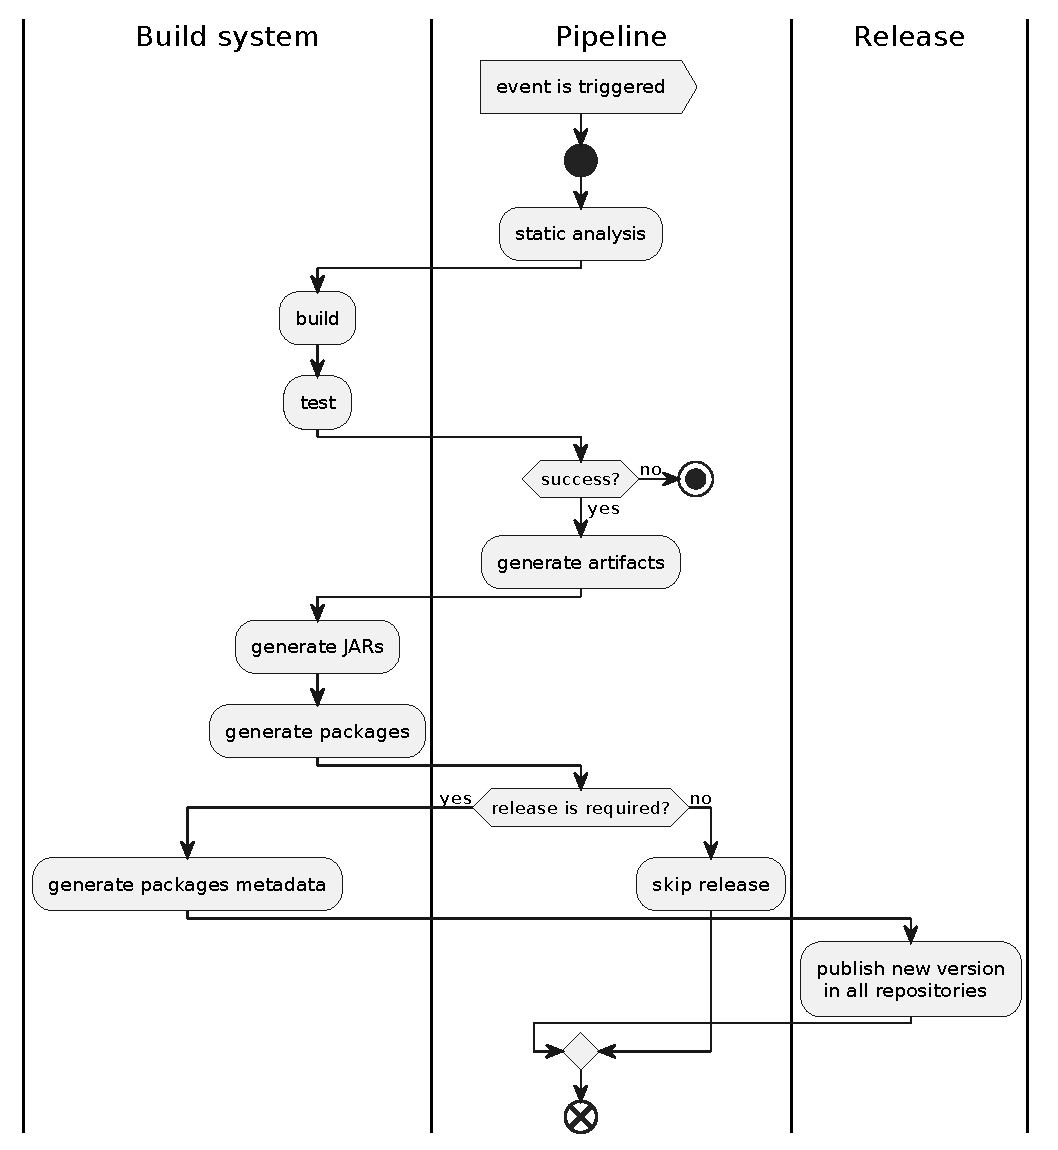
\includegraphics[width=.9\linewidth]{figures/activity-interaction-diagram.pdf}
	\caption{Diagramma delle attività raffigurante l'interazione tra i componenti}
	\label{fig:activity-interaction-diagram}
\end{figure}

Nello schema si fa riferimento ad un generico evento come segnale di avvio della pipeline. Nell'ambito \ac{cicd} l'evento corrisponde spesso alla pubblicazione di nuovo codice nel repository, in questo modo l'eventuale inserimento di errori viene rilevato e comunicato prontamente ai responsabili dello sviluppo del progetto.

\section{Build system}

Il ruolo principale del \textit{build system} è quello di esporre un \textit{task} adibito alla generazione dei pacchetti. Il task dovrà soddisfare i seguenti requisiti:
\begin{itemize}
	\item Deve configurare correttamente le opzioni di \textit{jpackage}, in particolare quelle che mutano nel tempo come la versione.
	\item È necessario stabilire un corretto ordine di esecuzione ed albero delle dipendenze per garantire la consistenza del processo.
	\item Deve consentire la dichiarazione di configurazioni differenti a seconda del sistema operativo che esegue il processo.
\end{itemize}

\subsection{JPackage}\label{sec:design-jpackage} Lo strumento \ac{cli} \textit{jpackage} offre un'interfaccia munita di diverse opzioni per configurare e personalizzare a piacimento i pacchetti in output. Esistono parametri generici, compatibili con tutte le piattaforme, e parametri specifici che vanno a modificare attributi particolari alla tipologia di pacchetto in output scelta. Uno dei motivi che ha portato alla scelta di \textit{jpackage} rispetto ad altri software è la capacità di includere autonomamente una \textit{runtime-image} di Java, ossia una \ac{jre} ridotta di dimensioni all'interno del pacchetto. La combinazione di una \textit{runtime-image} e degli archivi Java (JAR) necessari all'esecuzione dell'applicazione costituiscono l'\textit{application-image}: un pacchetto autocontenuto che include l'applicazione, assieme una \ac{jvm} ed alle librerie necessarie per eseguire quell'applicazione sulla piattaforma di destinazione.

\paragraph{Application image} Alchemist è un progetto modulare ed ogni modulo è distribuito in un archivio JAR specifico. Come descritto nella documentazione\footnote{https://alchemistsimulator.github.io/howtos/preparation/jar/index.html} il software predispone due modalità di utilizzo stand-alone attraverso l'esecuzione degli archivi Java. La prima modalità consiste nell'inclusione dei singoli moduli richiesti come \textit{classpath} del processo di esecuzione. La seconda modalità sfrutta l'archivio denominato ``full", ossia un \textit{fat-jar} contenente tutti i moduli e tutte le dipendenze necessarie all'esecuzione del software in tutte le sue parti. In ottica di ridurre le dimensioni del pacchetto e velocizzare il processo di impacchettamento, jpackage costruirà l'\textit{application-image} utilizzando quest'ultimo. La posizione ed organizzazione dei file è diversa a seconda della piattaforma di destinazione del pacchetto, il risultato dell'installazione in un ambiente Linux è descritto nella figura \ref{fig:activity-interaction-diagram}.  

\begin{figure}
	\centering
	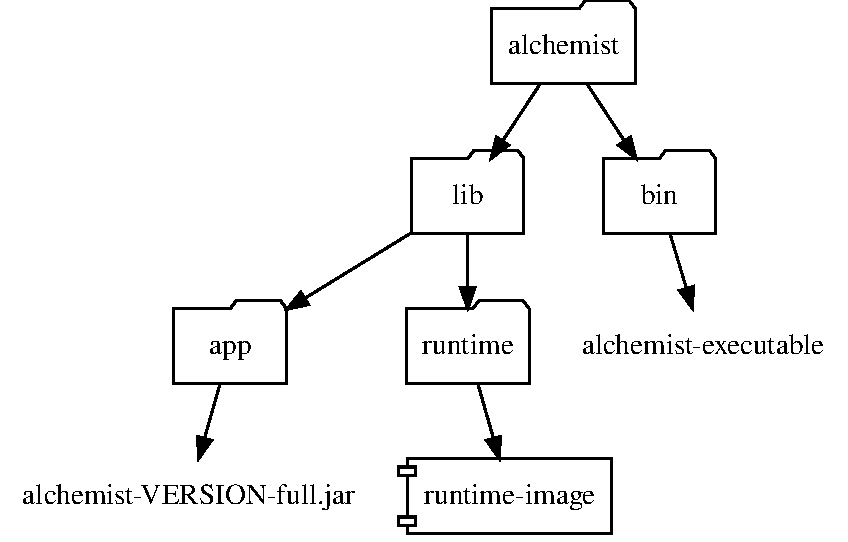
\includegraphics[width=.7\linewidth]{figures/application-image-folder-structure.pdf}
	\caption{Struttura del filesystem dell'\textit{application image} generato da \textit{jpackage} con Linux come piattaforma target}
	\label{fig:application-image-folder-structure}
\end{figure}

\paragraph{Integrazione} Per introdurre jpackage nel build system è necessario un task che funga da \textit{wrapper}: il quale esponga proprietà corrispondenti alle opzioni della \ac{cli} di jpackage. Gradle utilizza una pratica denominata \textit{lazy configuration} che fornisce la dichiarazione delle \textit{lazy properties} vale a dire ``proprietà pigre". Questa caratteristica consente di legare una proprietà ad un'altra senza doversi preoccupare dell'ordine di esecuzione. In tale modo non sono necessarie particolari attenzioni nell'assegnazione di proprietà come la versione, la quale viene calcolata da un plugin apposito. Il programma jpackage, come illustrato nella sezione \ref{sec:packaging}, non è \textit{cross-platform}, ciò significa che la generazione dei pacchetti deve essere eseguita su una macchina ospitante il sistema operativo di destinazione dei pacchetti richiesti. Per quanto lo strumento cerchi di unificare i diversi ambienti, ogni tipologia di pacchetto specialmente se di piattaforme diverse presenta limiti e regole differenti. Per questa ragione il task deve prevedere l'utilizzo di parametri differenti a seconda del sistema operativo sottostante.

\subsection{Design finale} Il design ultimo è raffigurato nella figura \ref{fig:gradle-jpackage-scheme}. 

\begin{figure}[htb]
	\centering
	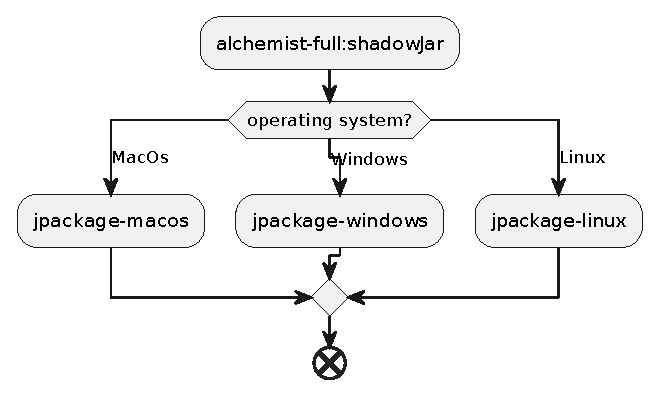
\includegraphics[width=.8\linewidth]{figures/gradle-jpackage-scheme.pdf}
	\caption{Diagramma delle attività rappresentante il processo di generazione dei pacchetti}
	\label{fig:gradle-jpackage-scheme}
\end{figure}
\noindent Come discusso nella precedente sezione il design divide la generazione nei tre sistemi operativi target e mantiene una dipendenza con \texttt{al\-che\-mi\-st\--fu\-ll\-:sha\-dow\-Jar\-}: il task incaricato di generare l'archivio JAR full.

\section{Pipeline}
La pipeline è l'elemento chiave per generare l'automazione dei processi descritti. Alchemist è già provvisto di una pipeline, la quale si occupa di analizzare il codice, verificare i processi di rilascio e in caso fosse necessario rilasciare una nuova versione. Il compito del design esplicato in questa sezione è quello di introdurre nuovi step con lo scopo di automatizzare la generazione e distribuzione dei pacchetti generati precedentemente. Le diverse unità di esecuzione o \textit{job} che popolano la pipeline possono essere distinti in base al loro ruolo.
\begin{itemize}
	\item \textbf{Inizializzazione}, tutte le unità incaricate di preparare l'ambiente di esecuzione della pipeline e quindi dei successivi job. 
	\item \textbf{Build e analisi}, i job responsabili di analizzare, compilare ed eseguire i test del codice.
	\item \textbf{Assemblaggio}, le unità di esecuzione responsabili della creazione di artefatti: archivi, pacchetti e documentazione.
	\item \textbf{Test}, job i quali verificano la validità degli artefatti o operazioni come la distribuzione.
	\item \textbf{Rilascio}, i componenti incaricati al rilascio di una nuova versione del software e le relative operazioni accessorie.
\end{itemize}

\begin{figure}[htb]
	\centering
	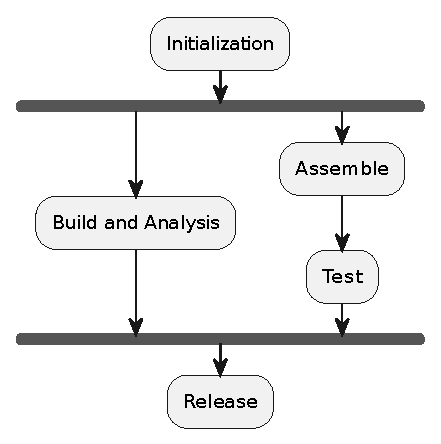
\includegraphics[width=.5\linewidth]{figures/pipeline-roles.pdf}
	\caption{Diagramma dell'attività illustrante il comportamento dei job all'interno della pipeline}
	\label{fig:workflow-roles-summary}
\end{figure}

Il flusso è in sintesi raffigurato nella figura \ref{fig:workflow-roles-summary}. L'\textbf{inizializzazione} trova spazio al primo posto e la sua esecuzione è strettamente necessaria per il proseguimento del flusso. L'\textbf{assemblaggio} e \textbf{build} sono eseguiti parallelamente mentre i \textbf{test} devono inevitabilmente dipendere dalla fase di assemblaggio per poter verificare l'output prodotto da quest'ultimo. Il \textbf{rilascio} infine, richiede che tutte le fasi descritte precedentemente siano eseguite con successo. I ruoli concernenti il lavoro descritto da questo elaborato sono: assemblaggio e test.

\subsection{Interazione con il Build System}
Per conseguire gli obiettivi dettati dai ruoli di assemblaggio e test è necessario l'utilizzo del build system. In particolare Alchemist sfrutta lo script \textit{gradle wrapper} per interagire con esso. Il file \textit{gradlew} è uno script che permette di eseguire Gradle senza doverlo installare globalmente: alla prima esecuzione controlla la versione richiesta definita in un file di configurazione, se quest'ultima non è presente allora il wrapper scarica questa e la utilizza per eseguire i task richiesti. I job, le unità di esecuzione della piattaforma GitHub Actions, consentono l'esecuzione di comandi nella \textit{shell} default (oppure una differente) del sistema operativo presente nel runner. In questo modo tramite comandi da shell è possibile eseguire lo script e fornire i task quali vogliamo eseguire come argomenti di questo.

\subsection{Test delle funzionalità}
Lo \textit{status} di un job indica il risultato dell'esecuzione di esso e può essere: \textit{failure}, \textit{success} oppure \textit{skipped}. Lo stato di un job è considerato in errore nel caso l'esecuzione di un comando restituisca un valore diverso da 0 e viceversa di successo nel caso restituisca 0, perciò non sono necessarie particolari funzionalità per implementare un processo di verifica. Lo stato \textit{skipped}, invece, si riferisce ai job non eseguiti secondo condizioni specifiche descritte dallo sviluppatore, è quindi possibile gestire un unico workflow e modificare il suo flusso a seconda dell'evento che ha innescato l'esecuzione. Il comportamento di default dello stato all'interno di una pipeline è bloccante per cui il fallimento di un job porta all'interruzione dell'intera pipeline, come raffigurato nel diagramma \ref{fig:activity-diagram-job}.

\begin{figure}[htb]
	\centering
	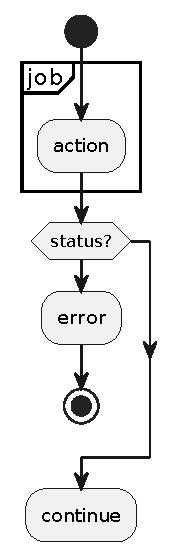
\includegraphics[width=.18\linewidth]{figures/activity-diagram-job.pdf}
	\caption{Diagramma dell'attività illustrante il processo attraverso i ruoli delineati}
	\label{fig:activity-diagram-job}
\end{figure}

\section{Release}

Un ultimo fattore fondamentale è il rilascio e la distribuzione del software. 

\subsection{Repository}

Ogni repository funziona attraverso tipologie di pacchetti diverse e processi di pubblicazione differenti. Di seguito saranno illustrate le regole vigenti nei vari citati in questo elaborato.

\paragraph{AUR}

\paragraph{WinGet}

\paragraph{Snapcraft}

\subsection{Conclusioni e punti comuni}

%Ad esempio il metodo del templating? 
%La presenza di uno script bash? 
%Le richieste necessarie nella pull-request?
%Esiste la possibilità di fare dei test? 